\section{Project Implementation}

To meet the initial requirements of the project statement, I structured my code around several classes to manage Thomas and his environment in a modular way.

\subsection{Architecture and Class Roles}
I adopted an object-oriented design based on an entity hierarchy, as illustrated in the following diagram:

\begin{figure}[H]
    \centering
    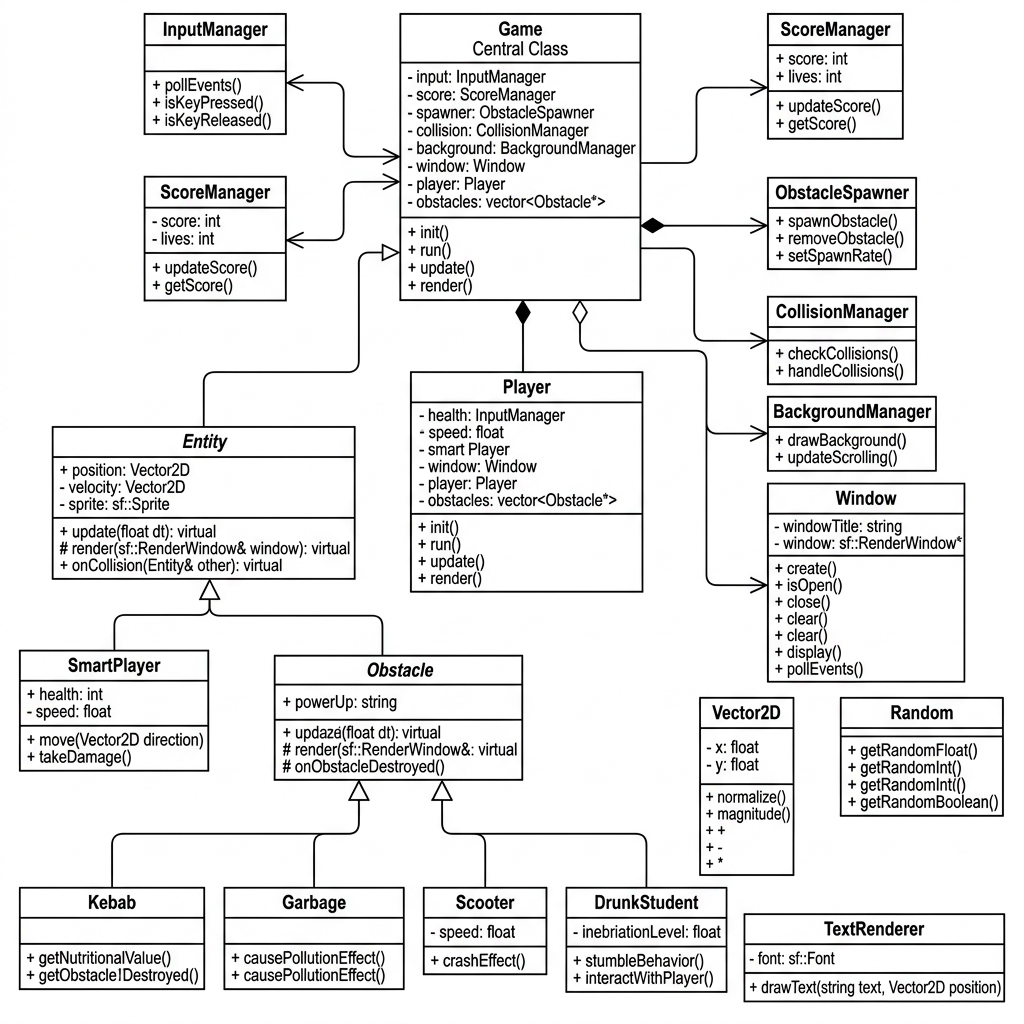
\includegraphics[width=0.7\textwidth]{images/class_diagram.png}
    \caption{Class diagram representing the project architecture.}
\end{figure}

\begin{itemize}
    \item \textbf{Entity}: Abstract base class defining common properties (position, size, velocity) and the virtual \texttt{update} and \texttt{draw} methods.
    \item \textbf{Player} and \textbf{Obstacle}: Specializations of \texttt{Entity}. Thomas and the various scrolling objects inherit from these classes to define their own behaviors.
    \item \textbf{Game}: Central class orchestrating the main loop and communication between different systems.
    \item \textbf{Management Systems}: Several specialized classes handle technical aspects: \texttt{InputManager} (keyboard/mouse), \texttt{ObstacleSpawner} (generation), \texttt{CollisionManager} (impact detection), \texttt{BackgroundManager} (parallax background), and \texttt{ScoreManager} (save management).
    \item \textbf{Utilities}: The \texttt{Vector2D}, \texttt{Random}, and \texttt{TextRenderer} classes provide cross-cutting tools for physics, randomness, and text display.
\end{itemize}

\subsection{Mandatory Features}
I implemented Thomas's movements as well as his "stagger" behavior (random zigzags). Health management is linked to screen brightness, and collisions trigger visual effects such as screen shake and temporary invincibility.

\begin{figure}[H]
    \centering
    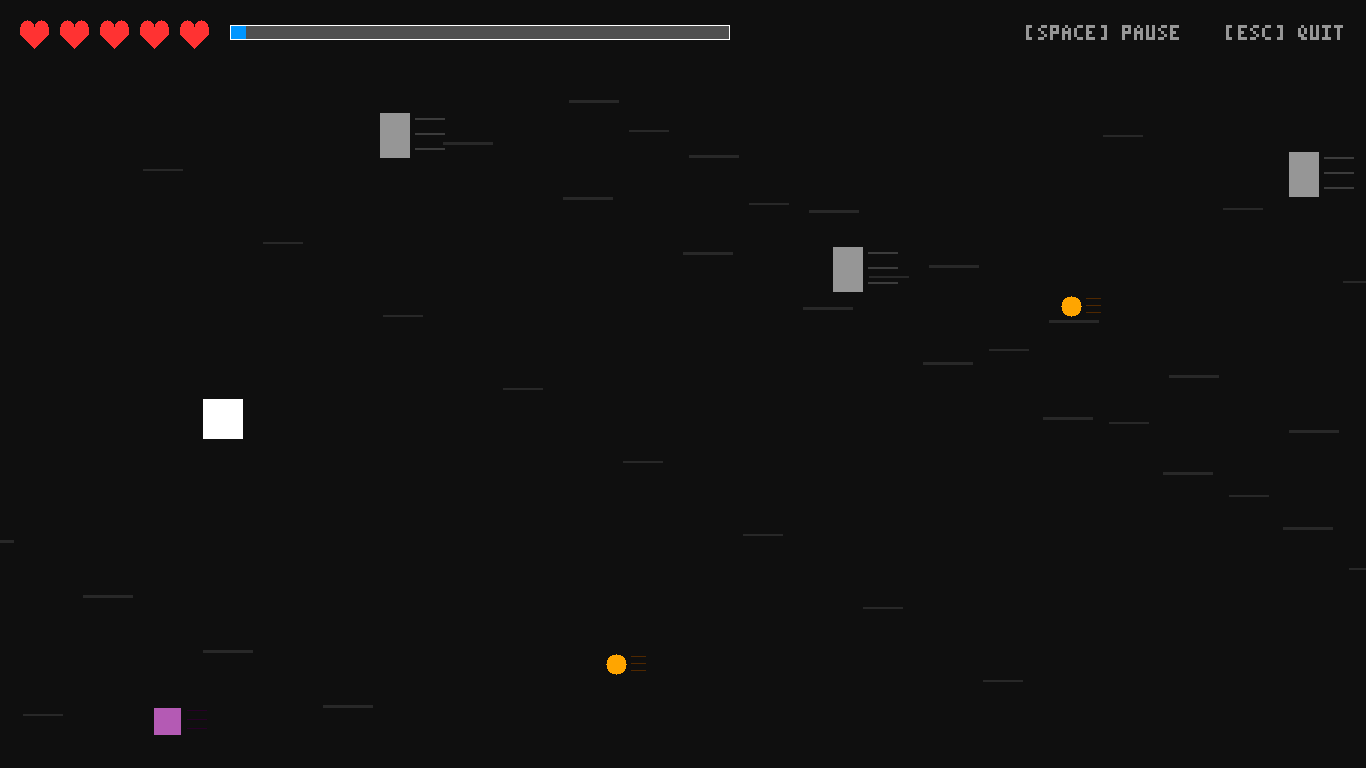
\includegraphics[width=0.6\textwidth]{images/playing.png}
    \caption{Thomas in-game avoiding obstacles.}
\end{figure}
